
%%%%%%%%%%%%%%%%%%%%%%% file typeinst.tex %%%%%%%%%%%%%%%%%%%%%%%%%
%
% This is the LaTeX source for the instructions to authors using
% the LaTeX document class 'llncs.cls' for contributions to
% the Lecture Notes in Computer Sciences series.
% http://www.springer.com/lncs       Springer Heidelberg 2006/05/04
%
% It may be used as a template for your own input - copy it
% to a new file with a new name and use it as the basis
% for your article.
%
% NB: the document class 'llncs' has its own and detailed documentation, see
% ftp://ftp.springer.de/data/pubftp/pub/tex/latex/llncs/latex2e/llncsdoc.pdf
%
%%%%%%%%%%%%%%%%%%%%%%%%%%%%%%%%%%%%%%%%%%%%%%%%%%%%%%%%%%%%%%%%%%%


\documentclass[runningheads,a4paper]{llncs}

\usepackage{amssymb}
\setcounter{tocdepth}{3}
\usepackage{graphicx}

\usepackage{url}
\urldef{\mailsa}\path|{ales.komarek, jakub.pavlik.7, vladimir.sobeslav}@uhk.cz|    
\newcommand{\keywords}[1]{\par\addvspace\baselineskip
\noindent\keywordname\enspace\ignorespaces#1}

\begin{document}

\mainmatter  % start of an individual contribution

% first the title is needed
\title{Ontology for OpenStack Service Architectures}

% a short form should be given in case it is too long for the running head
\titlerunning{Ontology for OpenStack Service Architectures}

% the name(s) of the author(s) follow(s) next
%
% NB: Chinese authors should write their first names(s) in front of
% their surnames. This ensures that the names appear correctly in
% the running heads and the author index.
%
\author{Ales Komarek\and Jakub Pavlik\and Vladimir Sobeslav}
%
\authorrunning{Lecture Notes in Computer Science: Authors' Instructions}
% (feature abused for this document to repeat the title also on left hand pages)

% the affiliations are given next; don't give your e-mail address
% unless you accept that it will be published

\institute{Faculty of Informatics and Management, University of Hradec Kralove,\\
Rokitanskeho 62, 50003 Hradec Kralove, Czech Republic\\
\mailsa\\
\url{http://cepsos.cz}}

%
% NB: a more complex sample for affiliations and the mapping to the
% corresponding authors can be found in the file "llncs.dem"
% (search for the string "\mainmatter" where a contribution starts).
% "llncs.dem" accompanies the document class "llncs.cls".
%

\toctitle{Lecture Notes in Computer Science}
\tocauthor{Authors' Instructions}
\maketitle


\begin{abstract}
%\boldmath

This paper explains how ontology can be used to model various OpenStack architectures. OpenStack is the largest open source cloud computing IaaS platform. It has been gaining wide spread popularity among users as well as software and hardware vendors over past few years. It's a very flexible system that can support a wide range of virtualization scenarios at any scale.

In our work we propose a formalization of OpenStack architectural model that can be automatically validated and serve suitable meta-data to configuration management tools. The OWL-DL based ontology defines service components and their relations and  provides foundation for further reasoning. Provided models can support simple all-in-one architecture as as well as large architectures with service components in High Availability setup.
\keywords{OpenStack, SOA, etc.}

\end{abstract}


\section{Introduction}

%proč OpenStack - protože komunita 500000 vývojářů, tisíce firem, nárůst kódu za poslední dobu stacalytics.com 

%vendor lockin, scalability from notebook to thousans of servers like CERN

OpenStack is the largest open-source cloud computing platform today. Many companies participate to its code, extend core functions and write new service backends to fit their business goals. The actual system consists of many components designed with plugin architecture that allows custom implementations for various service backends. These components can be combined and configured to match available software and hardware resources and real use-case needs.

Each implementation has its own component combination and use some form of configuration management tool to enforce the service states on designated servers and possibly other network components. These tools require data that covers configuration of all components. Detecting component inconsistencies by hand is painful and time consuming process.

We propose a formalization of OpenStack service architecture model, based on the approaches developed in classic knowledge representation domain, especially Service-Oriented Architecture by OpenGroup. Component definition is encoded in an ontology using the standard OWL-DL language, which enables sharing of knowledge about configurations across various systems. Reasoning can be used on the specification to automate validation of configuration changes.

When dealing with hundreds of components with thousands of properties and relations, keeping track of changes throughout its life cycle is very challenging. Current approaches are ad hoc, even OpenStack Fuel has severe limitations, there exists no standard for specifying common OpenStack architectural model. The question how to convert the proposed OWL-DL schema to metadata format that configuration management tools can process is discussed. We are working on external node classification service that uses graph database to serialize the OWL ontology with REST API that configuration management tools can use as metadata provider. This can streamline the process of adopting new services and service backends in predictable manner.

\begin{figure}[!h]
\centering
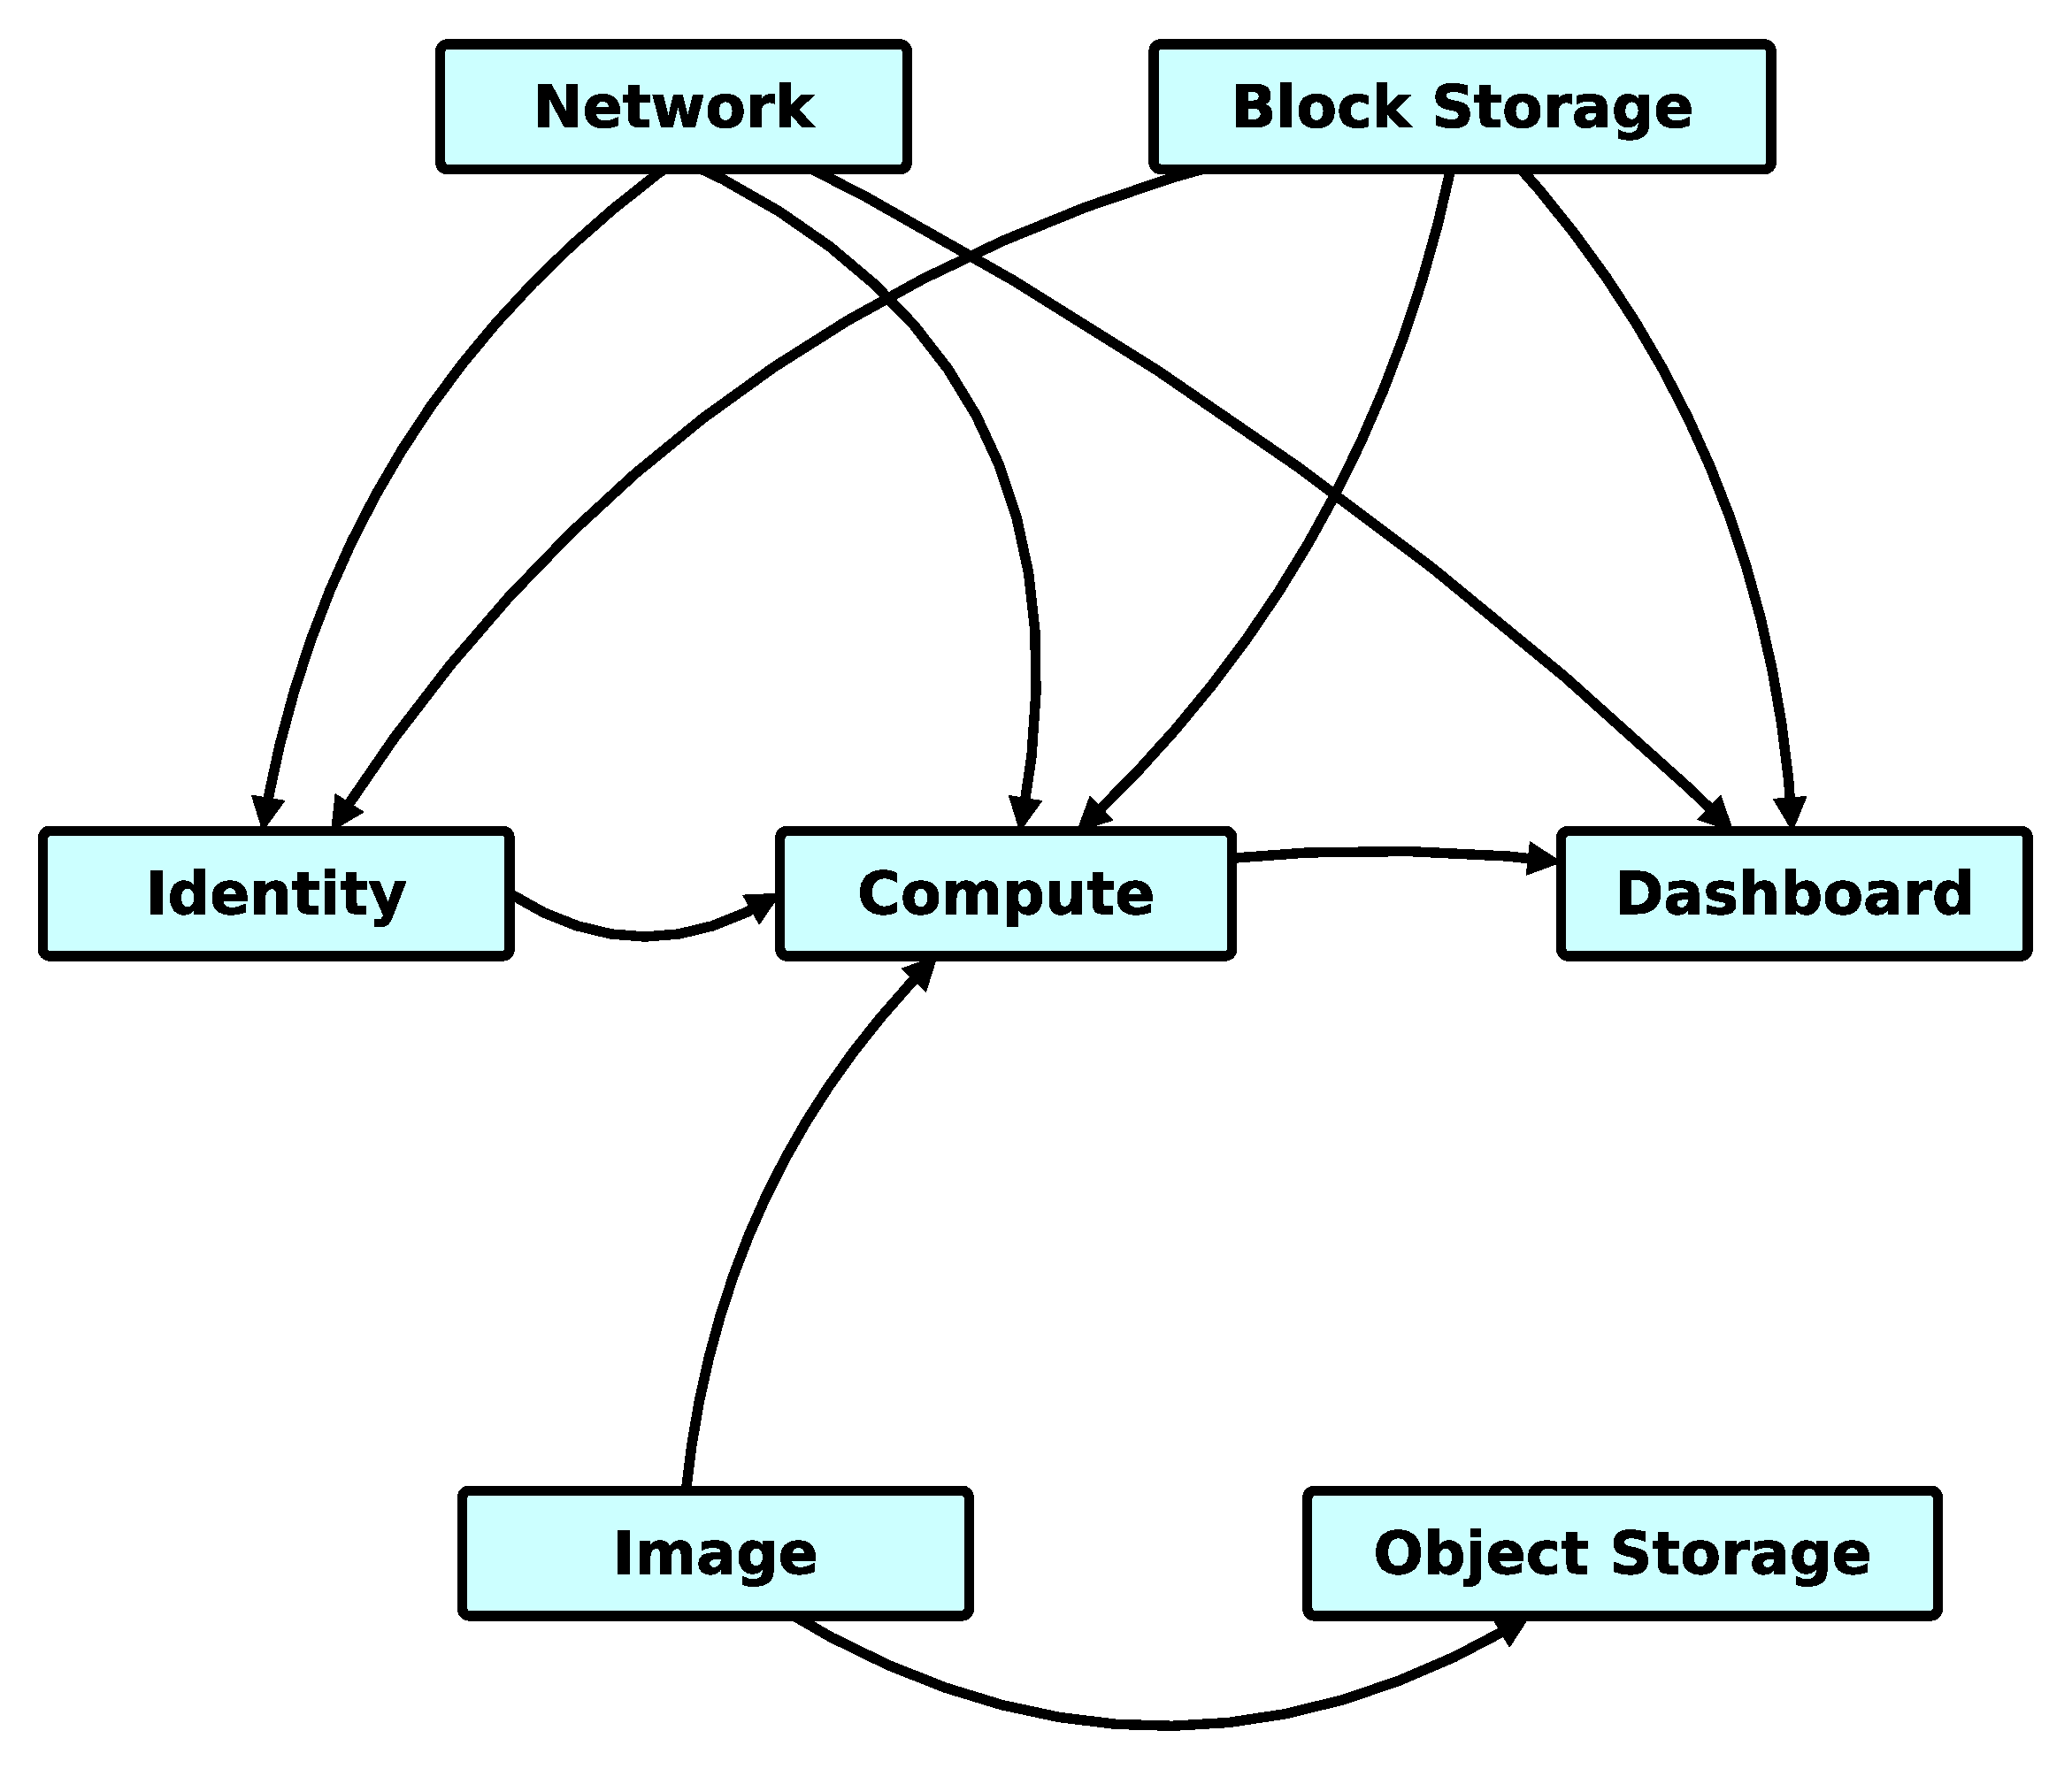
\includegraphics[scale=.2]{img/openstack_logical_model.eps}
\caption{Logical Model of Havana OpenStack}
\label{fig:cm}
\end{figure}


\begin{figure}[!h]
\centering
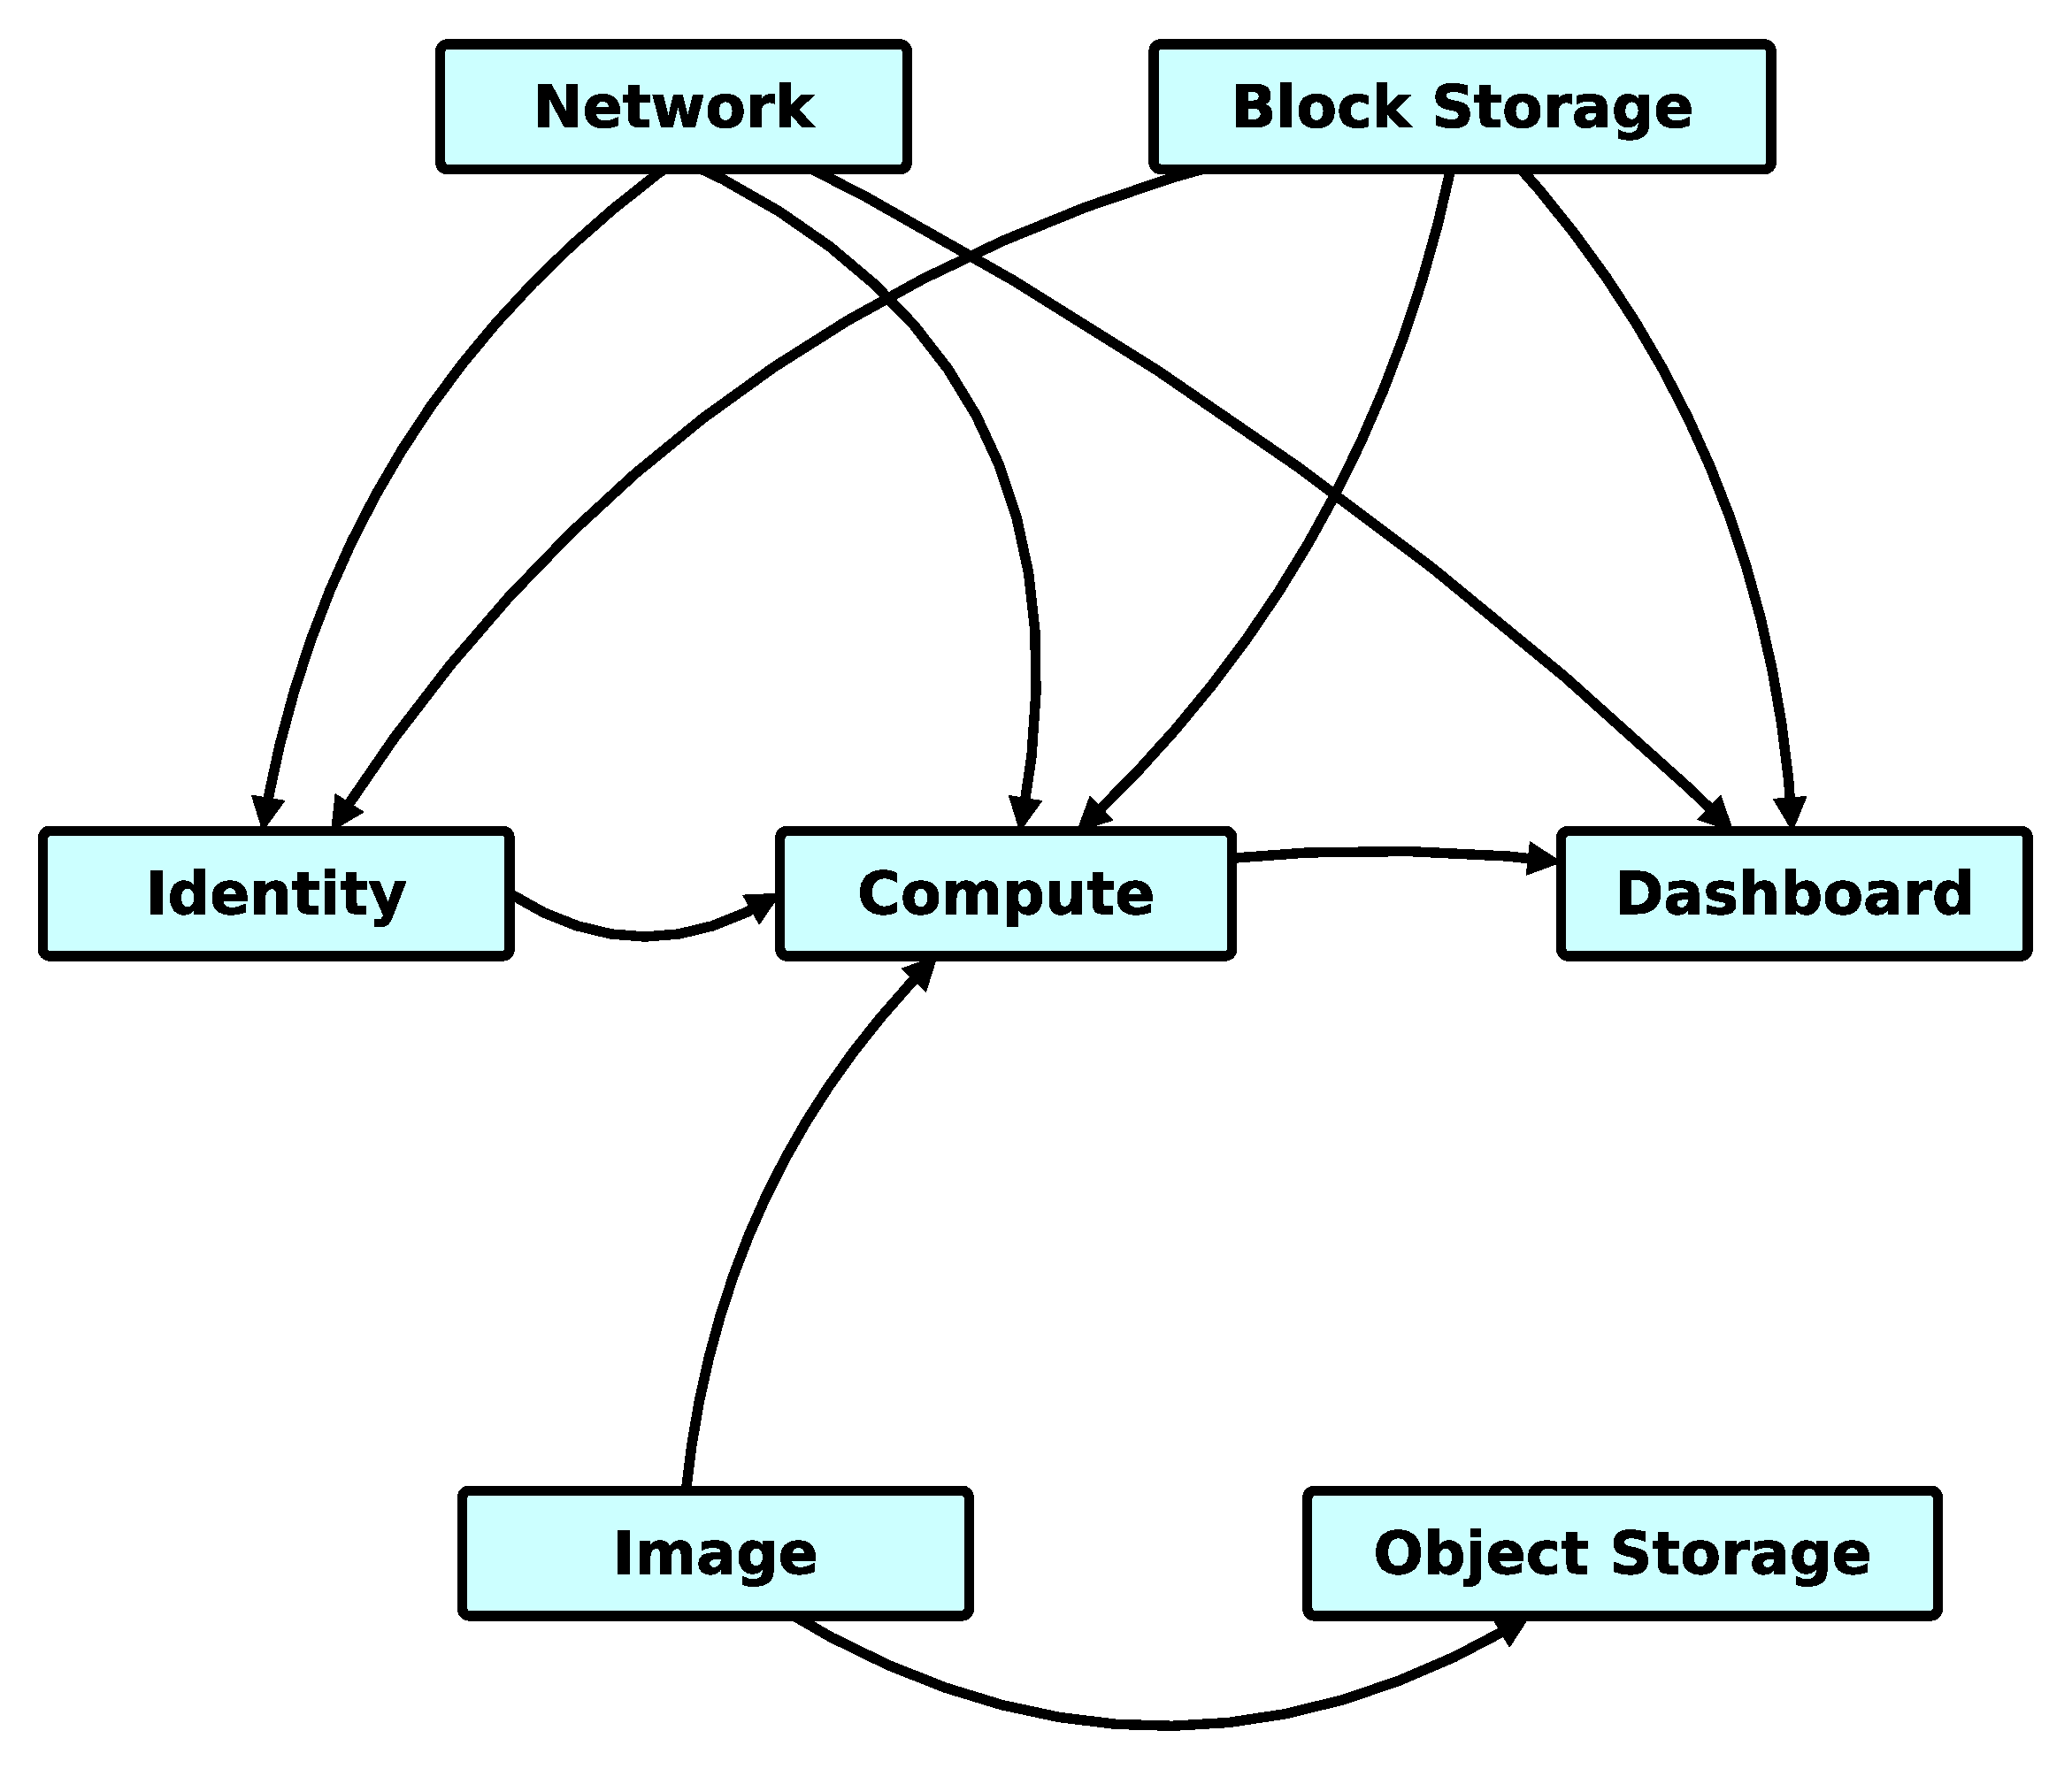
\includegraphics[scale=.2]{img/openstack_logical_model.eps}
\caption{Logical Model of Icehouse OpenStack}
\label{fig:cm}
\end{figure}


% představit OpenStack jako systém s rolemi, konfiguracemi, komponenty, drivery. jina instalace per use case. Nexexistuje univerzální instalace. Vysoka komplexita, services

% Jak vytvořit high level model (logické schéma) architektury? a přenést ji do low level design realizace? 
% Jak správně definovat architekturu na základě hw infrastruktury a target use case?

% Jak celý proces deploymentu automatizovat?

\subsection{IaaS Solutions}

\subsection{Use Cases}

\subsection{Infrastructure Modeling}


\section{SERVICE ARCHITECTURE MODELS}
\label{chap:service}


%Infrastructure as a Service platforms at it's core controls various virtualization interfaces and services and allows to launch a new virtual server from given disk image at chosen host server, connect it to provided physical or virtual network and add block storage device to it. The OpenStack platform provides services that address needed to provide the very basic compute, network and storage services. The identity provider and image store  provide further services needed to provide the basic sevices.
%Nebula was the predecessor of OpenStack and was superseded because it did not scale well. The services withing OpenStack communicate through 3 various communication channels
%TCP/SQL - Services store it's state in SQL datastore
%AMQP - Service internally communicate over asychronous communication bus which .... Compute service calls network service 
%HTTP - All services expose REST APIs that allow higher level integration, control ...

This section describes modularity and complexity of OpenStack IaaS platform including core and supporting services. However, there is not so much place for detail description of all components, since the main idea is contained in Sections \ref{chap:ontology} and \ref{chap:usage}. 
The goal of this section is to show that OpenStack modules are independent services, which can be implemented in many different of ways. 

\subsection{IAAS ARCHITECTURE CORE MODELS}

OpenStack is complete Infrastructure as a Service platform. It allows to create virtual servers on virtual networks using virtual block devices.

\begin{figure}[h]
\centering
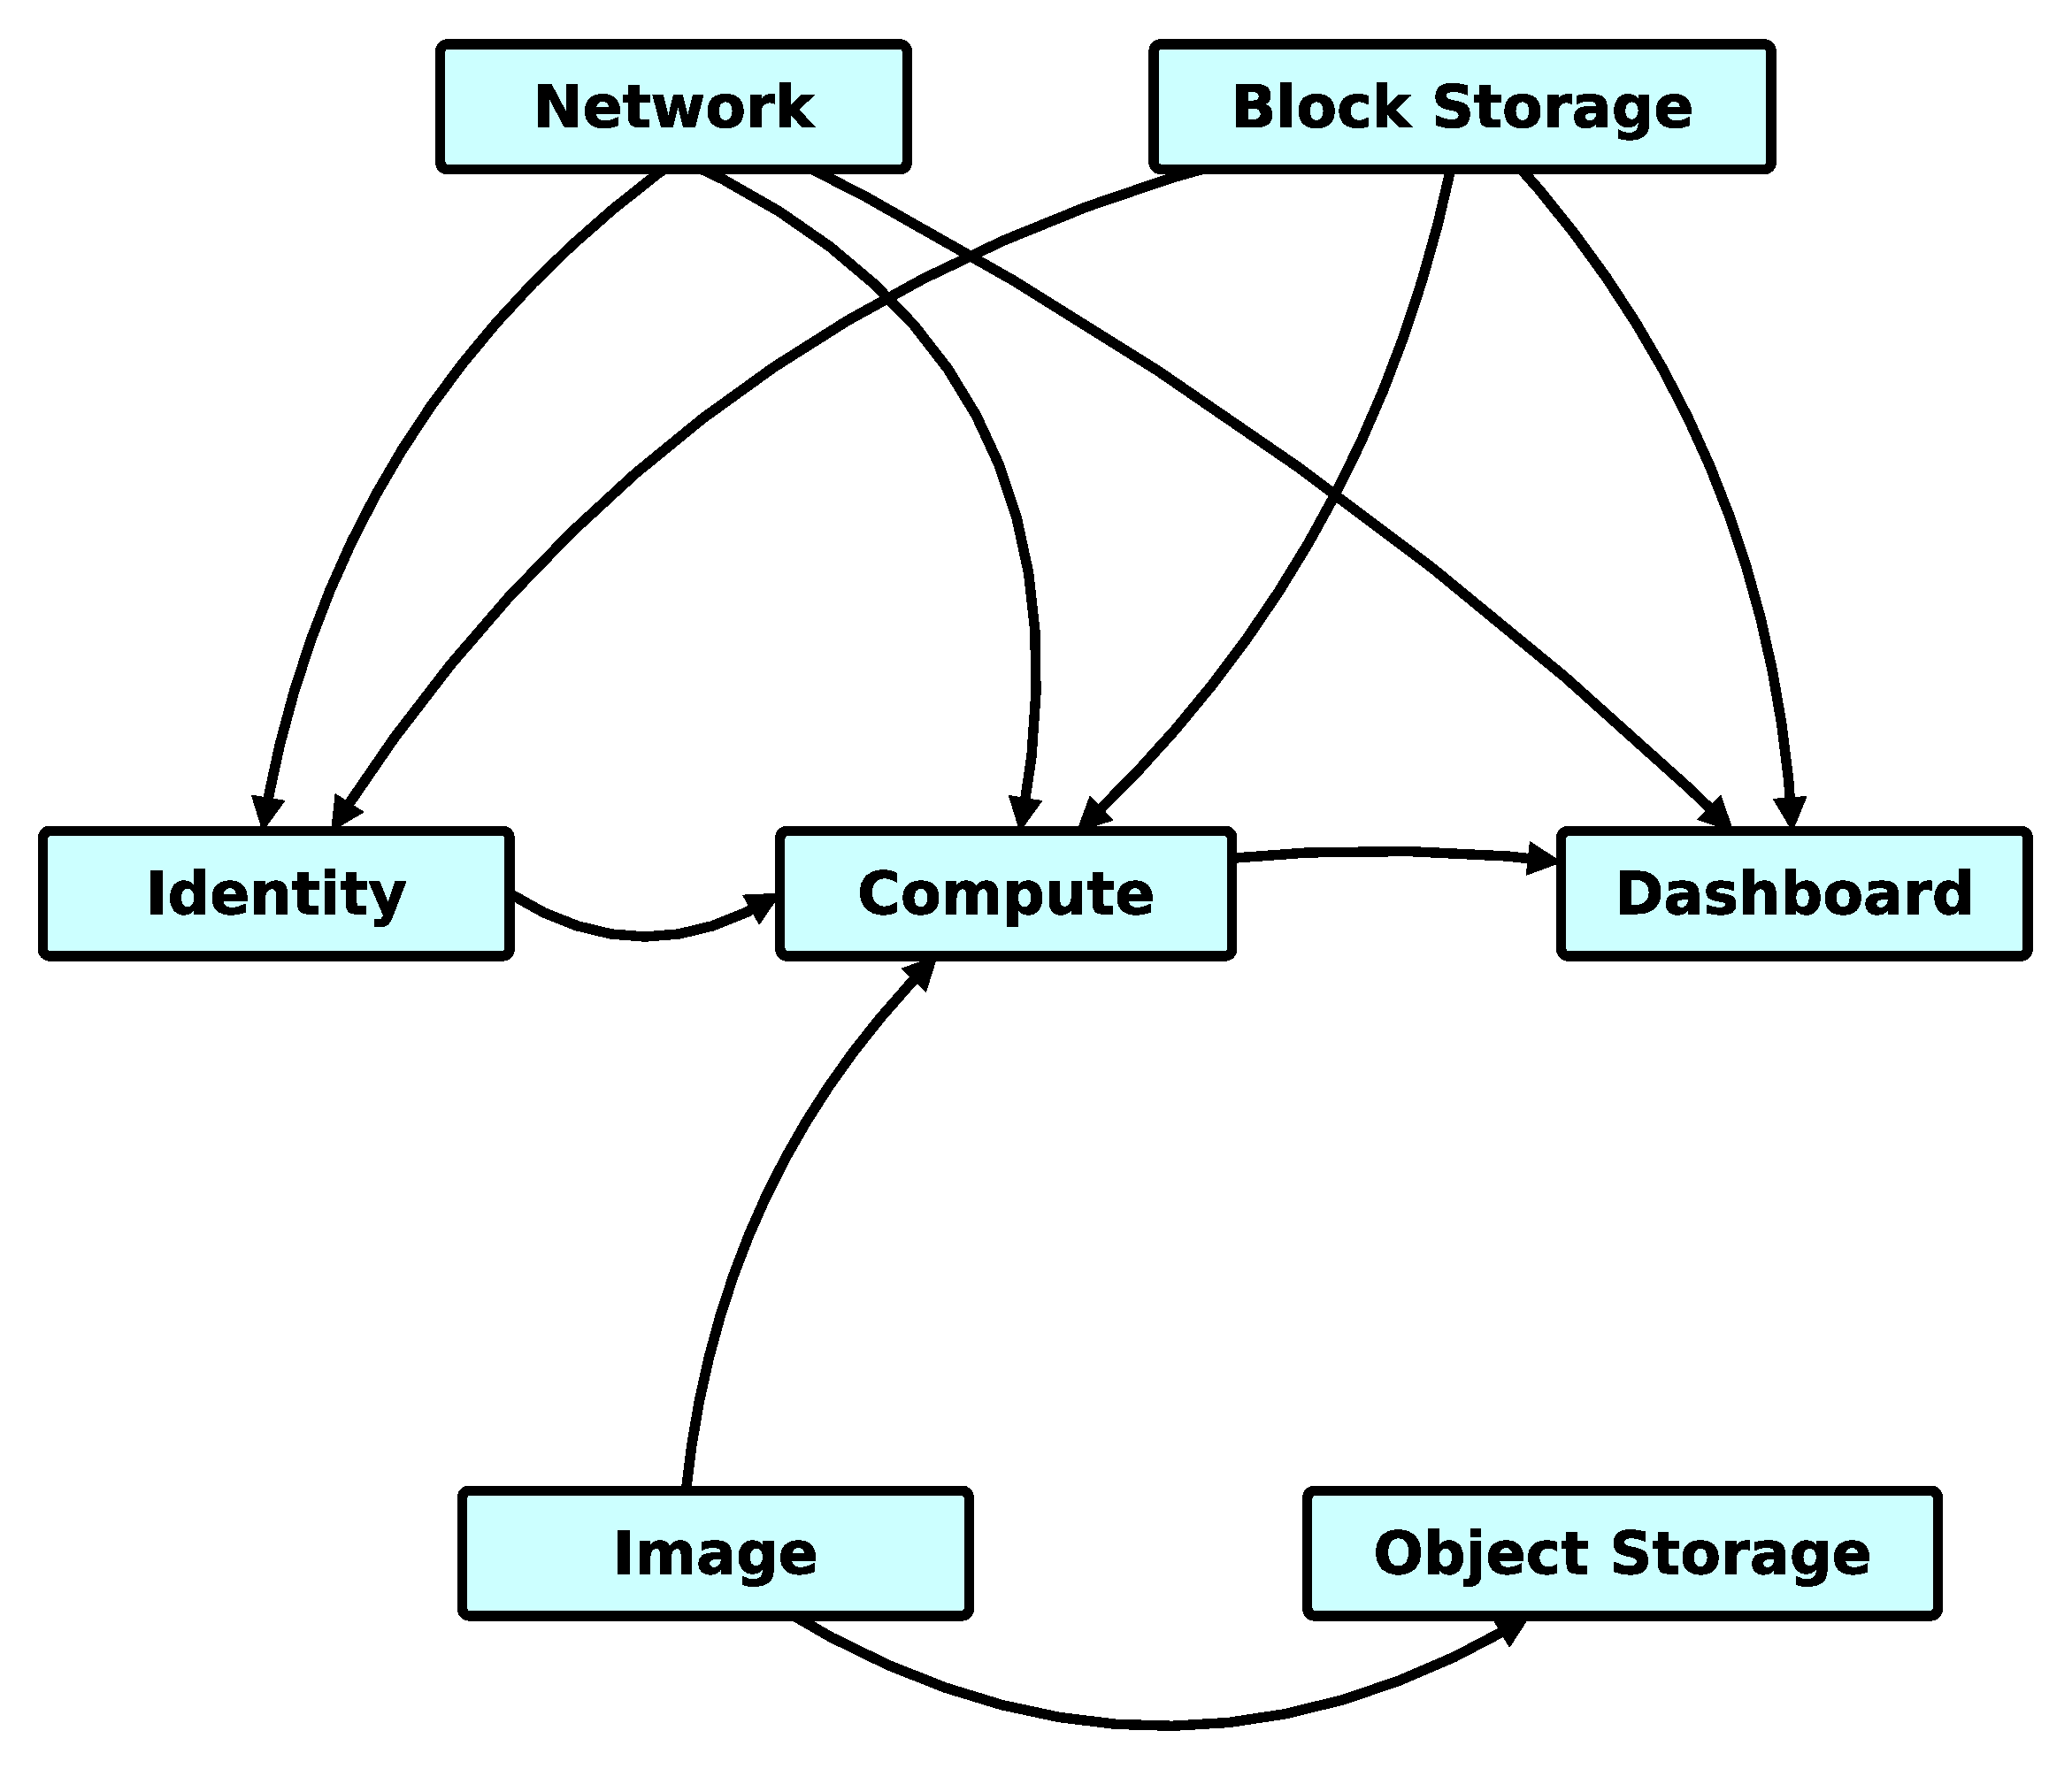
\includegraphics[scale=.13]{img/openstack_logical_model.eps}
\caption{Logical Model of Icehouse OpenStack service achitecture}
\label{fig:modules}
\end{figure}

\begin{figure}[!h]
\centering
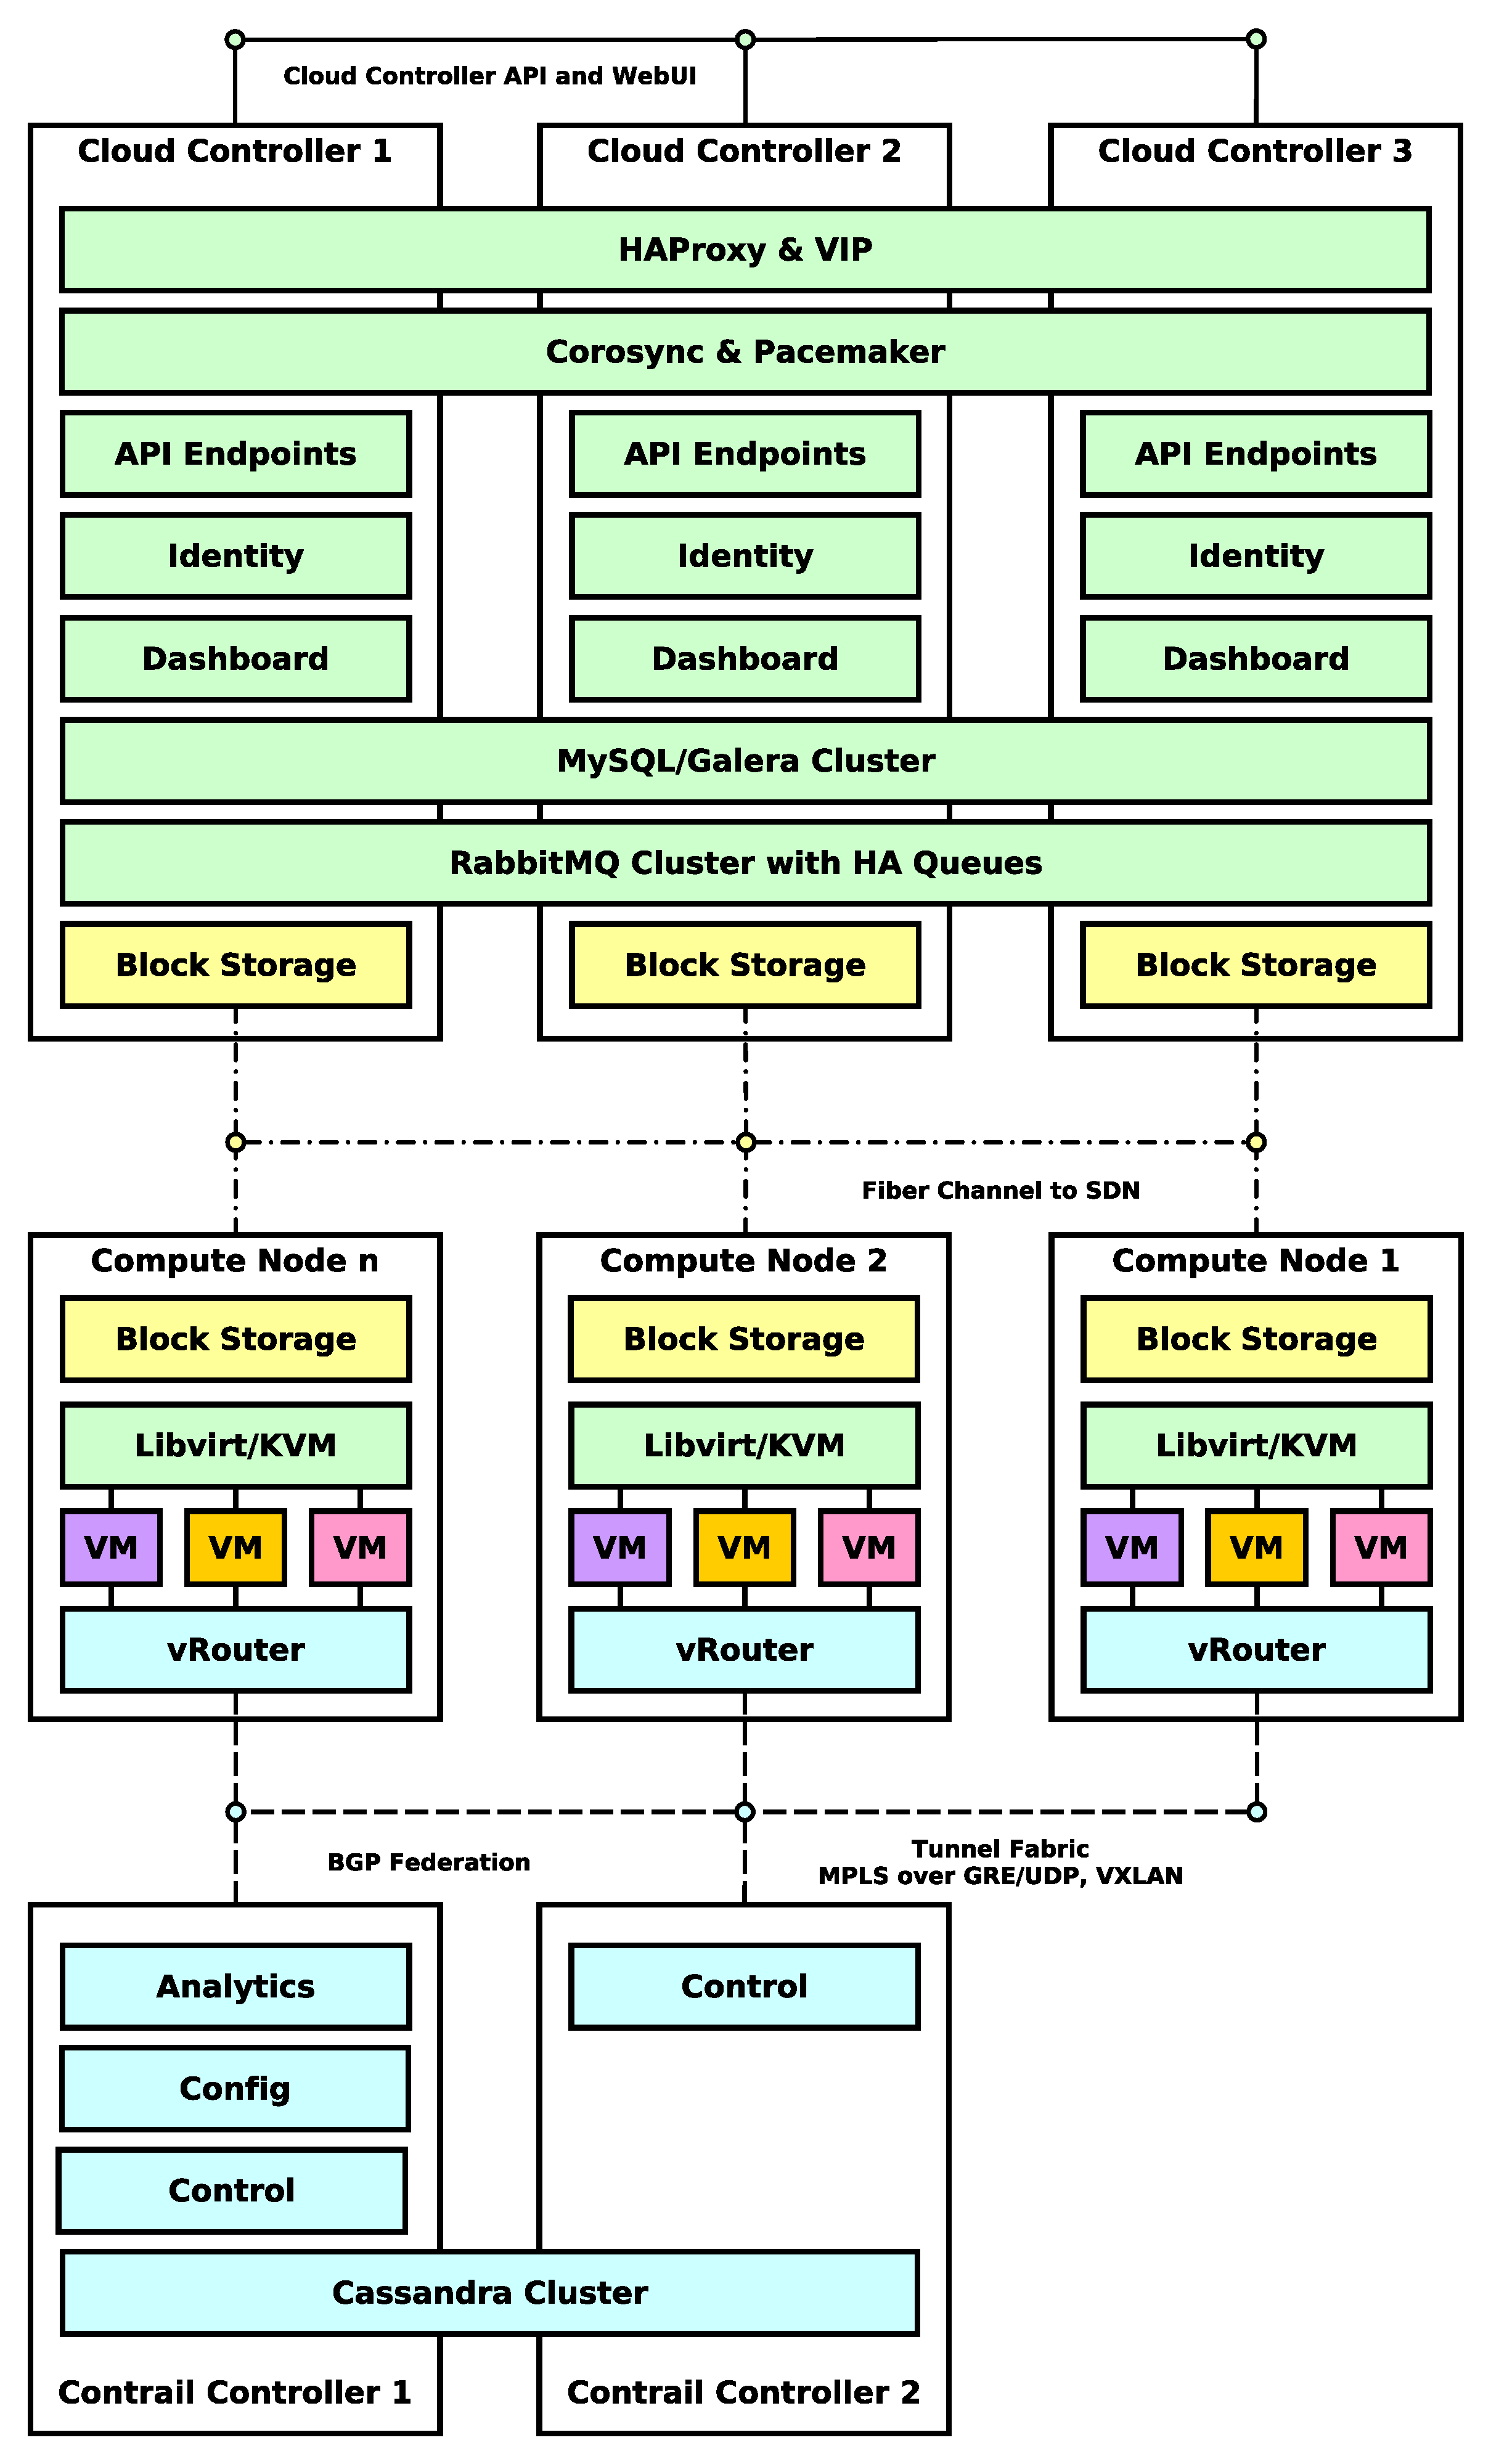
\includegraphics[scale=.15]{img/use_case_ha_sdn.eps}
\caption{Locality 2 Architecture}
\label{fig:pisek}
\end{figure}

%Jak funguje IaaS ve smyslu deploye masiny z pohledu controlleru - zavola scheduler, ten comupte, ten pak glance, pak pripadne cinder a neutron a pusti boot, kdyz to ma ready. a tim padem provoz.

Further versions of OpenStack introduce more complex services that use basic services to provide for example Data processsing, Database, Message Queue  or Orchestration. All services or modules within OpenStack architecture are independent and have pluggable backends or drivers. This allows vendors to develop plugin for their resources, that can be accessed and managed by the OpenStack API.

Fig. \ref{fig:modules} shows the core modules of OpenStack included in Icehouse release. Each module is briefly described including a serveral backends or plugins.


%Klasicky logicky model openstack architektury

%2) OpenStack architecture moduls

% Rozebrat services a představit modularitu a vendor plugins, drivers

\textbf{Identity - Keystone} is an OpenStack project that provides Identity, Token, Catalog and Policy services for use specifically by projects in the OpenStack family. 
\textit{Backends/plugins}: sql, ldap

\textbf{Image - Glance} service provides services for virtual disk images. Compute service uses image service to get the starting image of the virtual server.
\textit{Backends/plugins}: dir, Swift, Amazon S3

\textbf{Compute - Nova} service is designed to provision and manage large networks of virtual machines, creating a redundant and scalable cloud-computing platform. 
\textit{Backends/plugins}: KVM, Hyper-V, VMware vSphere, Docker

\textbf{Network - Neutron} is an OpenStack networking project focused on delivering networking as a service. It makes hard to deploy advanced networking services because of wide range of plugins.
\textit{Backends/plugins}: Nova flat networking, OpenVSwitch gre/vxlan, OpenContrail, VMware NSX, etc.

\textbf{Volume - Cinder} provides an infrastructure for managing volumes in OpenStack. It uses storage drivers for volumes direct mapping into virtual instances through FibreChannel or iSCSI. 
\textit{Backends/plugins}: LVM driver, SAN driver, EMC VNX, IBM Storwize, CEPH, Gluster, etc.

OpenStack is not only about its core services, but there are many services at infrastructural level that are essential as well.

\textbf{High Availability Cluster software} is responsible for clustering OpenStack services and creation High Availability in active/active or active/passive mode.
\textit{Backends/plugins}: corosync/pacemaker, keepalived

\textbf{Communication Service} is messaging between components of same OpenStack module.
\textit{Backends/plugins}: RabbitMQ, QPid, ZeroMQ

\textbf{Database Services} is responsible for storing persistent data of all modules.
\textit{Backends/plugins}: MySQL/galera, PostgreSQL

%Různé způsoby nasazení ukázky reálné architektury - promapovat ve 4 na ontologii

\subsection{USE CASES}

We participate in operations of several real OpenStack deployments in Central Eastern Europe. Each of them is different, which means that uses different backends in modules.
Because of lack of space we decided to show only one use case. Fig. \ref{fig:pisek} shows the logical architecture of TCP Virtual Private Cloud.

%\begin{figure}[!h]
%\centering
%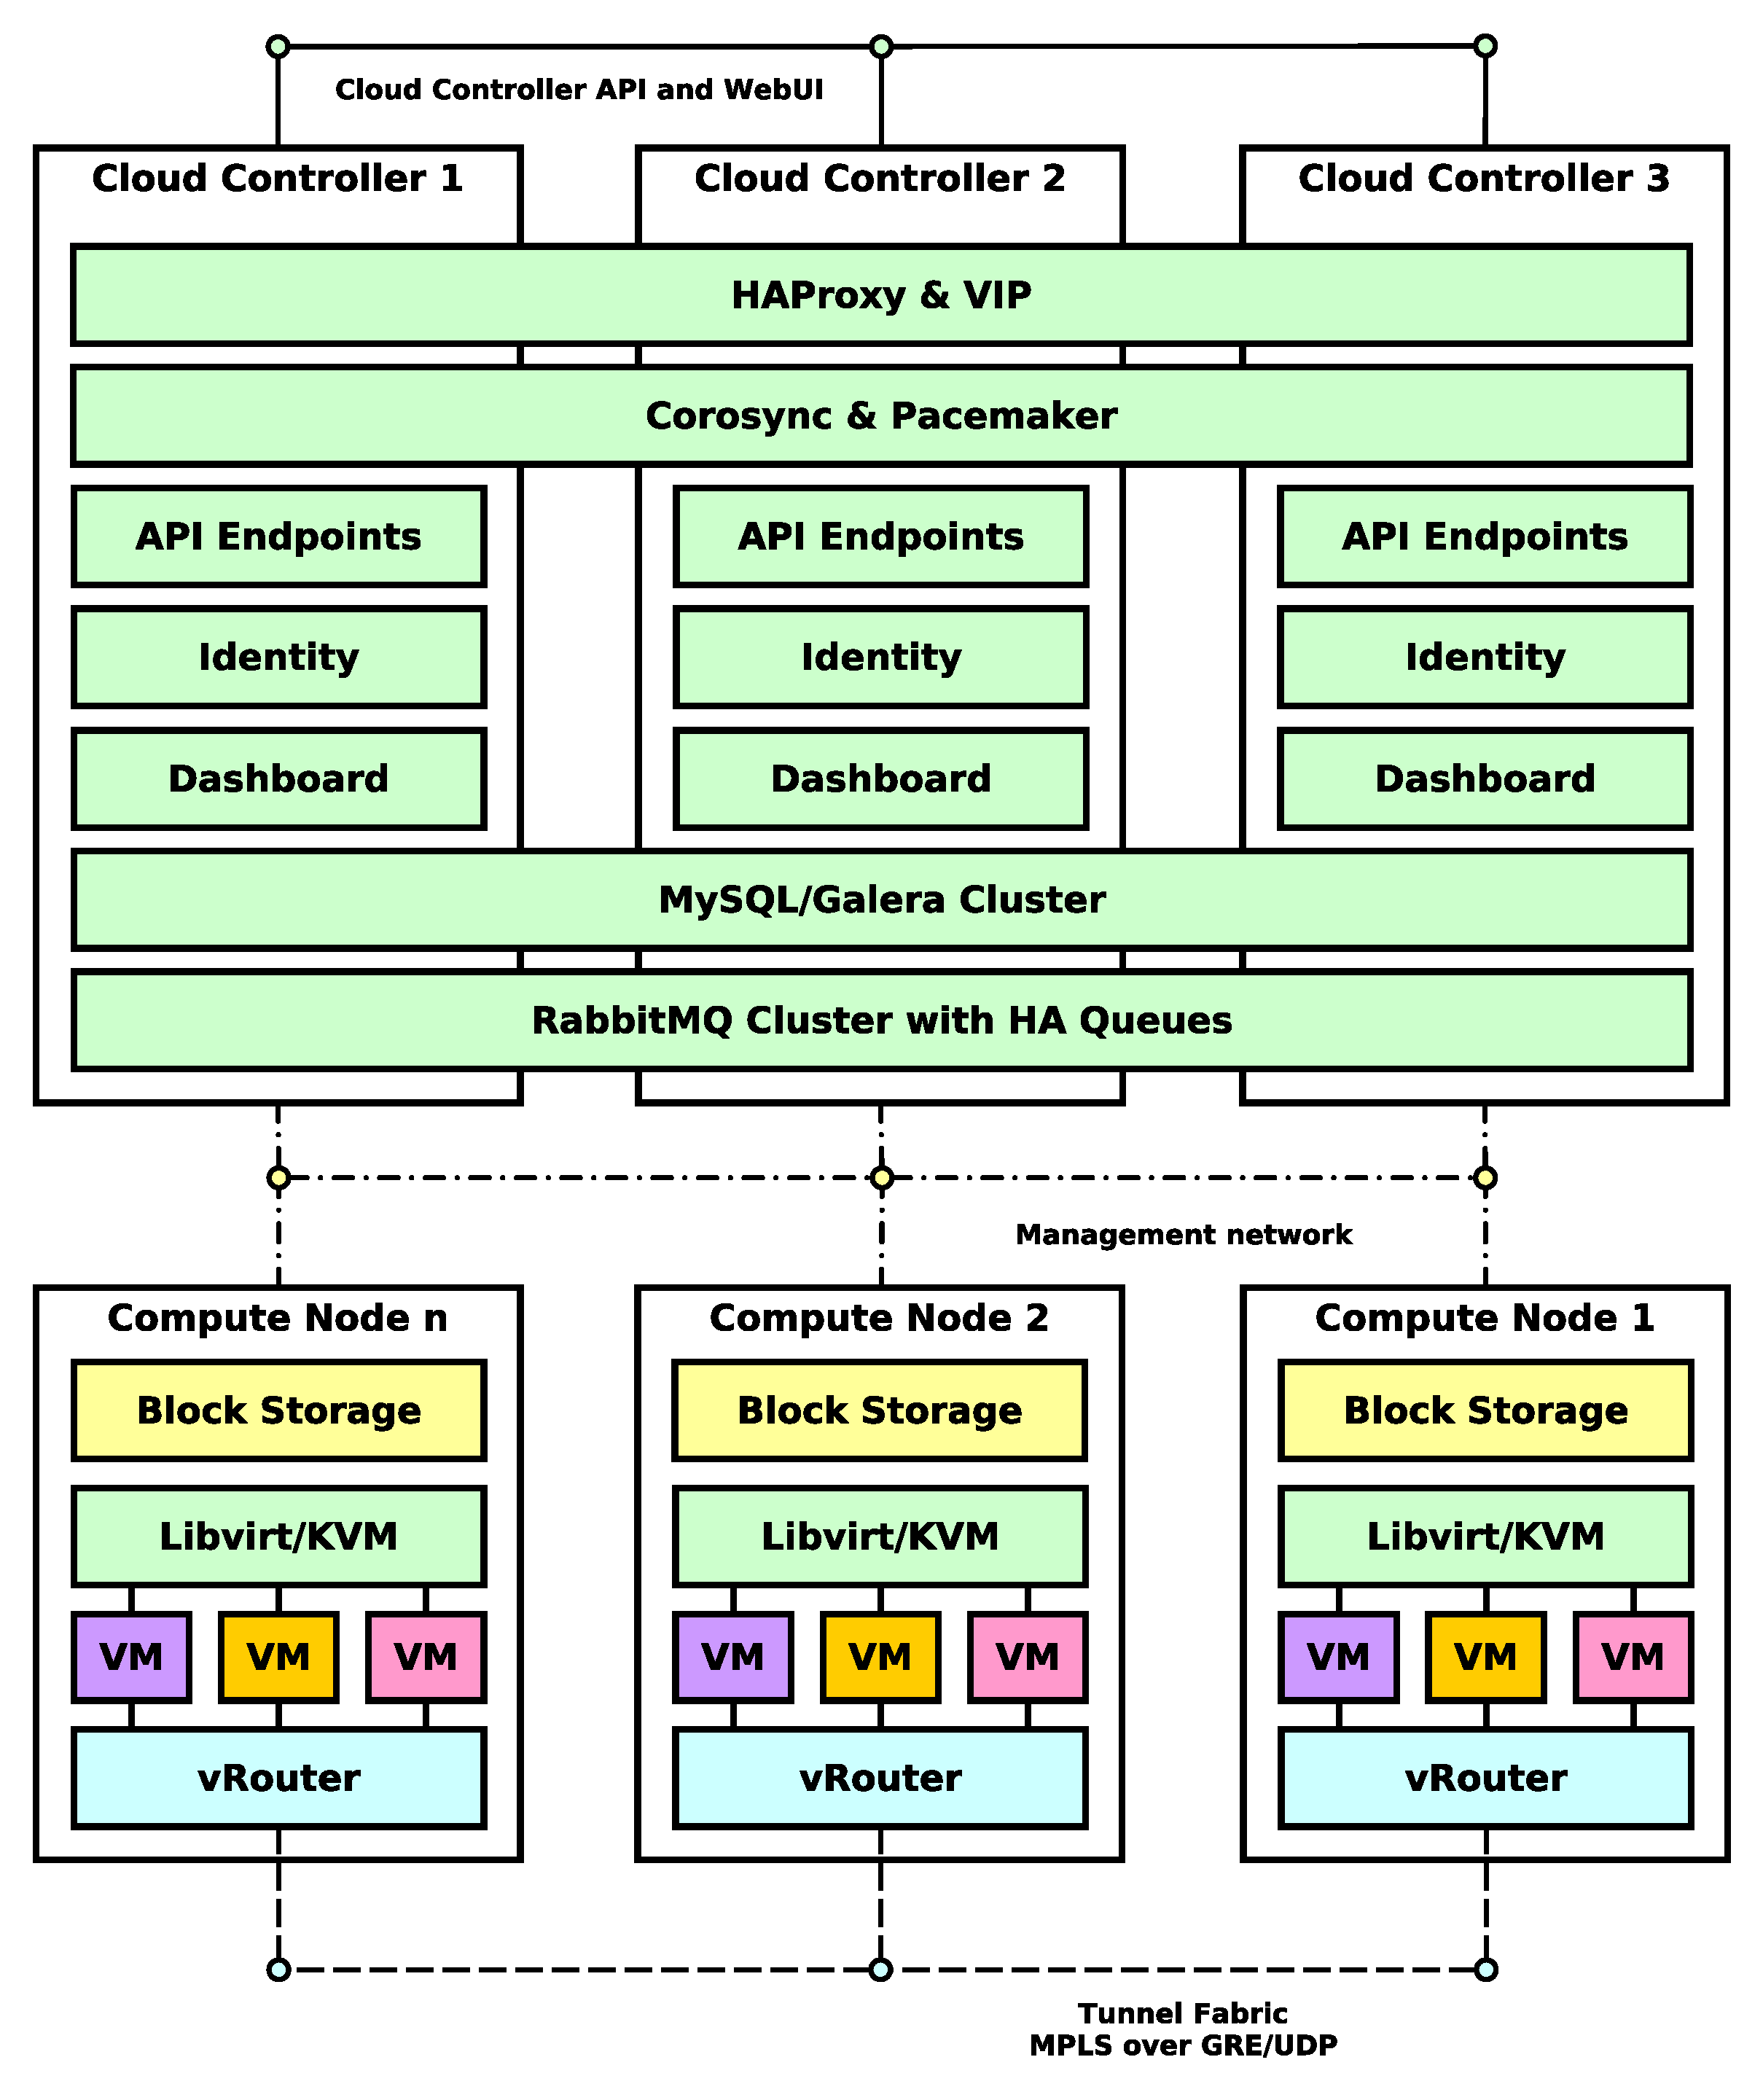
\includegraphics[scale=.2]{img/use_case_ha_gre.eps}
%\caption{Locality 1 Architecture}
%\label{fig:cm}
%\end{figure}

%\begin{figure}[!h]
%\centering
%\includegraphics[scale=.2]{img/use_case_l2_flat.eps}
%\caption{Locality 3 Architecture}
%\label{fig:cm}
%\end{figure}


\section{OpenStack Deployment Tools}

There are many ways how to deploy OpenStack infrastructure which are more or less automated. Some of them require to fill in answer files, some configuration files. Some tools have graphiceal user interface and allow to provision entire hardware infrastructure as some just configure the services on the provisioned servers.

Model je popsanej dokumentem a není to čitelný, automatizace. Není validita modelu. Chyby se debugují na úrovni reality.

\begin{figure}[!h]
\centering
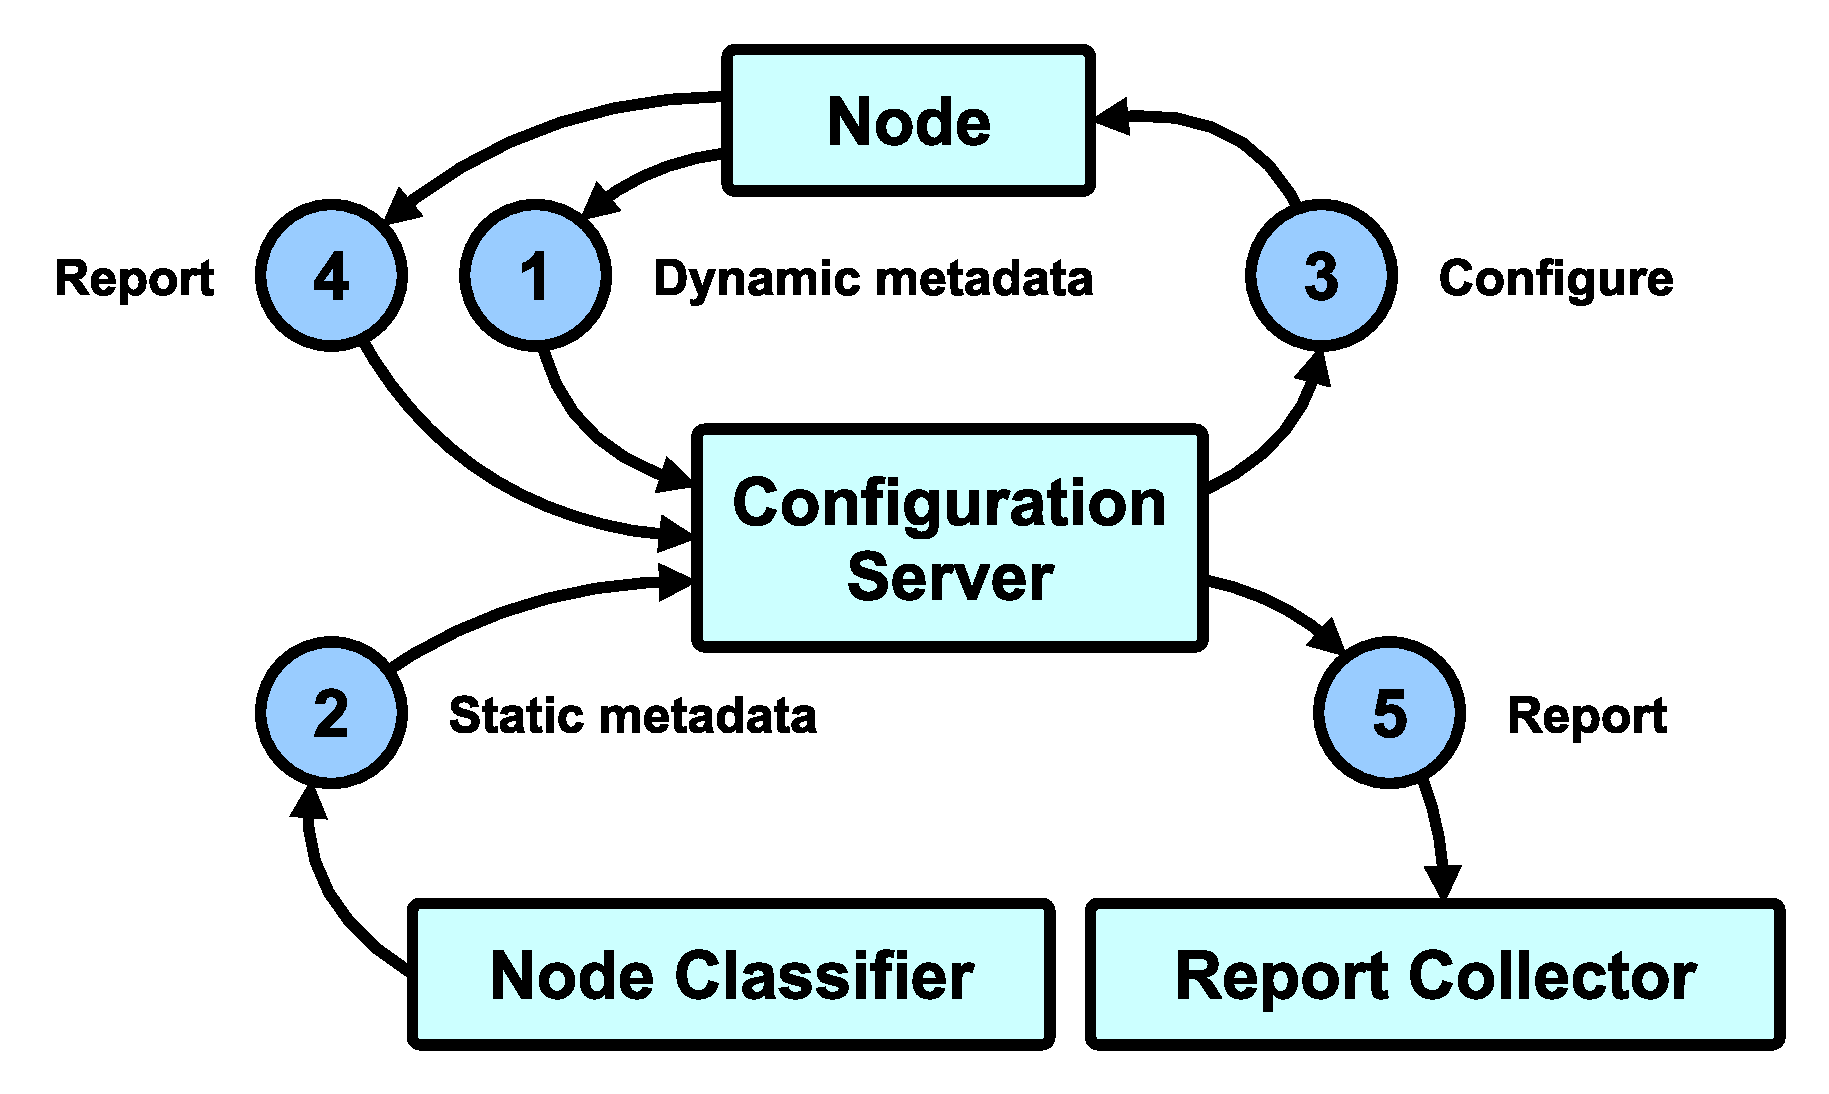
\includegraphics[scale=.15]{img/cm_cycle.eps}
\caption{Configuration Management deployment cycle}
\label{fig:cm}
\end{figure}


\subsection{Development}

For testing and developing OpenStack ...

\subsubsection{PackStack}

\subsubsection{Devstack}

\subsection{Production}

\subsubsection{Fuel}

\subsubsection{Foreman}


\section{OpenStack Platform Ontology}

Let's start what the ontology is, the short is answer:

    An ontology is a specification of a conceptualization. 

The broader answer may be:

	In the context of computer and information sciences, an ontology defines a set of representational primitives with which to model a domain of knowledge or discourse.  The representational primitives are typically classes (or sets), attributes (or properties), and relationships (or relations among class members). The definitions of the representational primitives include information about their meaning and constraints on their logically consistent application.

There formal definition exists

Servers (physical and virtual)

Core Infrastructure Services (DNS,DHCP,NTP, image management)

Storage (NAS and SAN)

Network (Routers, Switches, Firewalls, Load Balancers)

Facilities (Power, Cooling, Space)

\subsection{Standard Ontologies}

The ontologies define the relations between terms, but does not prescribe exactly how they should be applied. 

\subsubsection{Service-Oriented Architecture}

The SOA ontology specification was developed in order to aid understanding, and potentially be a basis for model-driven implementation of software systems

The ontology is represented in the Web Ontology Language (OWL) defined by the World-Wide Web Consortium (W3C). OWL has three increasingly expressive sub-languages: OWL-Lite, OWL-DL, and OWL-Full [OWL]. This ontology uses OWL-DL, the sub-language that provides the greatest expressiveness possible while retaining computational completeness and decidability.

The ontology contains classes and properties corresponding to the core concepts of SOA. The formal OWL definitions are supplemented by natural language descriptions of the concepts, with graphic illustrations of the relations between them, and with examples of their use. For purposes of exposition, the ontology also include.

\subsubsection{OSLC Configuration Management}



\subsection{Serialization Formats}

Způsoby serialiazce ontologie

\subsubsection{XML Documents}

RDF format

\subsubsection{Graph databases}

Preserving RDF format, just very different implementation 

je to servica, tzn overhead oproti xml filu, ale zas ma api atd ...

\subsubsection{Hierarchical}

Subject (id) or property driven

\subsection{Comparison}

Srovnání jednolivých formátů pro ontologii pro openstack řešení - bezpečnost, rychlost, integrace

- speed - parsing / scaling

- integration, maintenance costs

- security issues


\section{Ontology Usage}

% ontologie mohou dobre popsat openstack architekturu, protoze openstack vyuziva message bus, service catalog. Ontologie slouzi pak nad ramec openstack sluzeb u serveru ale definuji i vlastni operacni systemy a pridruzene sluzby - monitorting, metering, firewally, backupy, log management atd

We started mapping the very

% ontologie je multiregionalni podporuje vice lokaci najednou

The Ontology can support many individual implementations at the time

%

\subsection{Implementation details}

% Vytvorerin ontologie - protoege, na zaklade SOA ontologie
% testovani reasoningu pres pellet vyvozovani

Initial work on creating our Ontology was done in Protege, open-source ontology editor and framework for building intelligent systems.

The ontology is transformed into graph database using our python-bases service named django-ENC that can read and write ontology from OWL-DL XML files created by Protege and communicates with neo4j graph database through REST API. The graph databases are part of family of NoSQL databases and offer much better performance at any volume of data.

\begin{figure}[!h]
\centering
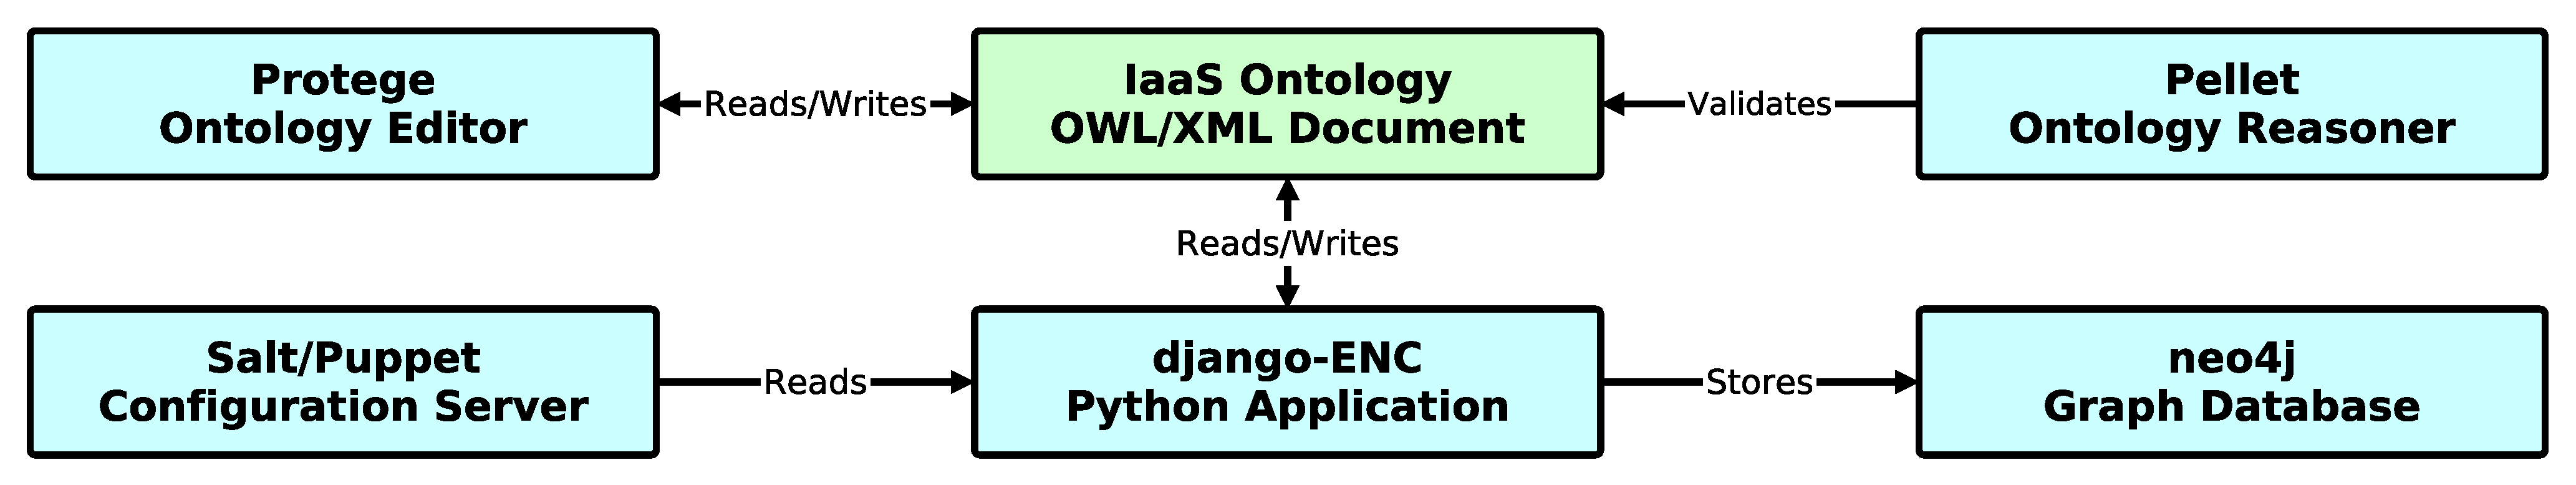
\includegraphics[scale=.17]{img/django_enc_arch.eps}
\caption{Ontology Service Architecture}
\label{fig:cm}
\end{figure}

The django-ENC service  use  web framework Django to deliver web services and asynchronous task queue Celery to perform time consuming tasks like ontology assertions and synchronizations between XML and graph database. Service expose it's owns HTTP REST API that can be consumed by configuration management tools like Salt or Puppet through their External Node Classification option.

The metada passed to CM tools is valid for 1st level of Cloud computing ontology [cite] 

%

We have tested SaltStack configuration management tool to instantiate 

The process is not yet fully automated as there is need of setting up network and storage components manually, but the progress in both configuration management tools and network and storage will allow better automation of these components by on-place agents or access protocols like SSH.

\subsection{Ontology samples}

Given use case scenario Lab1 we have 3 virtual servers providing OpenStack and core services in HA mode. These servers are virtualised in common . 20 physical servers  

\subsubsection{Service components of controller1}

\begin{lstlisting}
  <owl:Class rdf:about="#Glance">
    <owl:disjointWith>
      <owl:Class rdf:about="#"/>
    </owl:disjointWith>
    <owl:disjointWith>
      <owl:Class rdf:about="#ServiceInterface"/>
    </owl:disjointWith>
    <rdfs:subClassOf>
      <owl:Class rdf:about="#Composition"/>
    </rdfs:subClassOf>
  </owl:Class>
\end{lstlisting}

\subsubsection{Detail of service glance.image}

\begin{lstlisting}
  <owl:Class rdf:about="#Glance">
    <owl:disjointWith>
      <owl:Class rdf:about="#"/>
    </owl:disjointWith>
    <owl:disjointWith>
      <owl:Class rdf:about="#ServiceInterface"/>
    </owl:disjointWith>
    <rdfs:subClassOf>
      <owl:Class rdf:about="#Composition"/>
    </rdfs:subClassOf>
    <owl:disjointWith>
      <owl:Class rdf:about="#ServiceInterface"/>
    </owl:disjointWith>
    <rdfs:subClassOf>
      <owl:Class rdf:about="#Composition"/>
    </rdfs:subClassOf>
  </owl:Class>
\end{lstlisting}

\subsubsection{Detail of data property type}

\begin{lstlisting}
  <owl:Class rdf:about="#Glance">
    <owl:disjointWith>
      <owl:Class rdf:about="#"/>
    </owl:disjointWith>
    <owl:disjointWith>
      <owl:Class rdf:about="#ServiceInterface"/>
    </owl:disjointWith>
    <rdfs:subClassOf>
      <owl:Class rdf:about="#Composition"/>
    </rdfs:subClassOf>
  </owl:Class>
\end{lstlisting}

\subsubsection{Detail of object property database}

\begin{lstlisting}
  <owl:Class rdf:about="#Glance">
    <owl:disjointWith>
      <owl:Class rdf:about="#"/>
    </owl:disjointWith>
    <owl:disjointWith>
      <owl:Class rdf:about="#ServiceInterface"/>
    </owl:disjointWith>
  </owl:Class>
\end{lstlisting}


\section{Conclusion}

We have managed to do the first step to formalize and use IaaS Service Ontology to alleviate system operators tasks. The ontology can be used to create and validate meta-data for individual OpenStack installations. The generated meta-data is used to set-up variety of services from core, maintenance to actual OpenStack services. 

The ontology is  

Ontologická reprezentace prostředí, která je vhodná pro agentové prostředí, aby bylo možné provádět autonomní rozhodnutí. 

\subsection{Future work}

In the future we plan expand mapping ontology to network and storage resources in addition to servers with configuration tools. Ontology model is suitable for software agent processing and their rational decisions. It is possible to define processes that will maintain the configuration of real services in accordance to model systems.

\begin{thebibliography}{4}


% http://ryandlane.com/blog/2014/08/04/moving-away-from-puppet-saltstack-or-ansible/

% http://ryandlane.com/blog/2014/08/26/saltstack-masterless-bootstrapping/


% Cloud computing definitions

\bibitem{NIST}
\newblock {\em  NIST. The NIST Definition of Cloud Computing}
\newblock http://csrc.nist.gov/publications/nistpubs/800-145/SP800-145.pdf

\bibitem{CloudServices}
Ivan Ivanov, Marten van Sinderen and Boris Shishkov, editors.
\newblock {\em Cloud Computing and Services Science }
\newblock Springer Science, 978-1461423256, New York, USA, 2012

% ontological standards

\bibitem{OntologyDefinition}
\newblock {\em Encyclopedia of Database Systems }
\newblock Ling Liu and M. Tamer Özsu (Eds.), Springer-Verlag, 2009.

\bibitem{OWL}
\newblock {\em Web Ontology Language (OWL) }
\newblock http://www.w3.org/2004/OWL


\bibitem{SOAOntology}
\newblock {\em Service-Oriented Architecture Ontology, Version 2.0 }
\newblock ISBN:  1-937218-50-8, The Open Group, 2014

\bibitem{OasisCM}
\newblock {\em Configuration Management Resource Definitions }
\newblock http://open-services.net/wiki/configuration-management/Configuration-Management-Resource-Definitions/

\bibitem{DCMITerms}
\newblock {\em DCMI Metadata Terms }
\newblock http://dublincore.org/documents/dcmi-terms/

\bibitem{OBO}
\newblock {\em The Open Biological and Biomedical Ontologies  }
\newblock http://www.obofoundry.org/

\bibitem{ODA}
\newblock {\em Ontology Driven Architectures and Potential Uses of the Semantic Web in Systems and Software Engineering }
\newblock http://www.w3.org/2001/sw/BestPractices/SE/ODA/

% ontological applications

\bibitem{Pellet}
\newblock {\em Pellet: OWL 2 Reasoner for Java }
\newblock http://clarkparsia.com/pellet/

% Cloud computing deployment tools and config management tools

\bibitem{OpenStackFuel}
\newblock {\em OpenStack. Fuel Wiki }
\newblock https://wiki.openstack.org/wiki/Fuel

\bibitem{DevStack}
\newblock {\em Fedora Project. OpenStack devstack}
\newblock http://fedoraproject.org/wiki/OpenStack\_devstack

\bibitem{Cfengine}
\newblock {\em CFEngine. FCEngine 3.5 Documentation }
\newblock https://cfengine.com/docs/3.5/index.html

\bibitem{Foreman}
\newblock {\em The Foreman. The Manual: Compute Resources }
\newblock http://theforeman.org/manuals/1.4/index.html

% Metadata storage and retreival systems

\bibitem{ReClass}
\newblock {\em reclass. Recursive external node classification }
\newblock http://reclass.pantsfullofunix.net/

\bibitem{PuppetHiera}
\newblock {\em Puppet Labs. Creating Hierarchies }
\newblock http://docs.puppetlabs.com/hiera/1/hierarchy.html



\end{thebibliography}


\end{document}
